\chapter{Návrh riešenia}
\label{kap:navrh} % id kapitoly pre prikaz ref


\section{Návrh ontológie}

\begin{figure}[h]
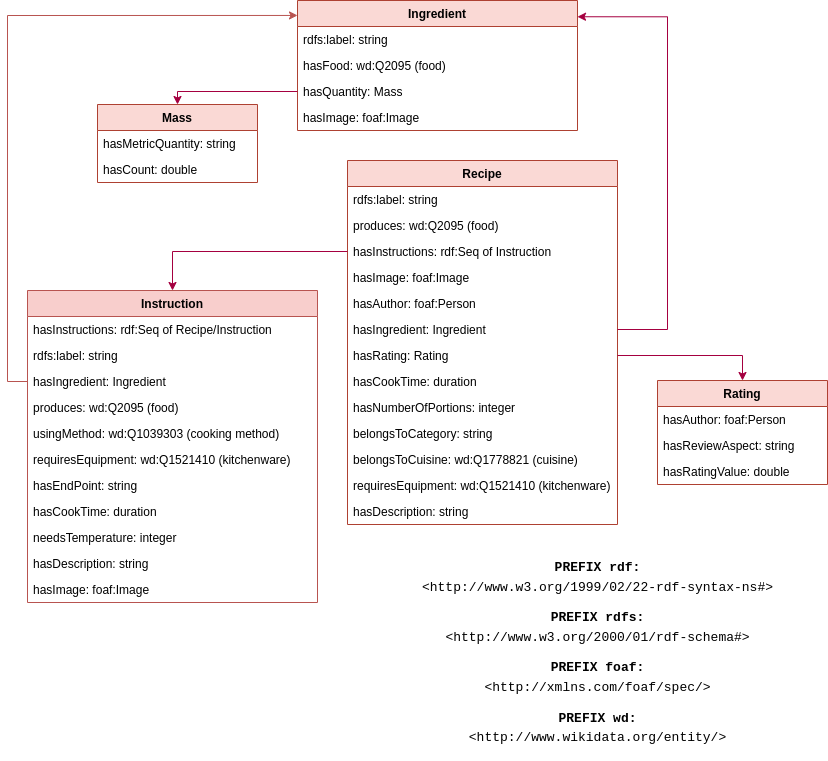
\includegraphics[width=\textwidth]{images/ontology}
\caption{Grafické vyjadrenie návrhu ontológie o receptoch}
\label{ontology}
\end{figure}

\subsection{Protégé}
Na vytvorenie ontológie sme využili Protégé, ktorý je možné stiahnuť na stránke \href{https://protege.stanford.edu/}{https://protege.stanford.edu/}. Protégé poskytuje grafické používateľské rozhranie, je to voľne dostupný editor ontológií a framework pre budovanie inteligentných systémov. Umožňuje modelovať triedy, predikáty, či vytvárať obmedzenia na jednotlivé predikáty. Následne je možné uložiť takto vytvorenú ontológiu v niektorej zo syntaxí pre jazyk OWL. Pri tvorbe našej ontológie sme využívali túto základnú funkcionalitu.

\subsection{Existujúca ontológia}
	Naša ontológia nadväzuje na ontológiu o receptoch v minuloročnej bakalárskej práci \cite{bakalarka}. Hlavnou úlohou bolo rozšíriť pôvodnú ontológiu o triedu, respektíve triedy, ktoré budú reprezentovať jednotlivé kroky (inštrukcie) v postupe receptu, keďže predtým bol postup iba pole reťazcov. V priebehu tvorby ontológie však došlo aj k ďalším menším zmenám v existujúcich triedach. Zároveň boli z pôvodnej ontológie odstránené triedy ingredientList a Food. Trieda ingredientList iba zapuzdrovala všetky ingrediencie patriace ku konkrétnemu receptu a trieda Food, ktorá vyjadrovala už existujúcu triedu a v našom prípade nebolo potrebné k nej pridávať žiaden ďalší predikát.
	
\subsection{Navrhnutá ontológia}
Nižšie je popísaná ontológia podľa obr. \ref{ontology}. Pri popisovaní ontológie je v zátvorkách uvedený presný názov predikátu tak, ako sa nachádza v ontológií a v jej grafickom vyjadrení na obr. \ref{ontology}. V pravom dolnom rohu obr. \ref{ontology} sú uvedené využité prefixy v prípade, že trieda alebo predikát boli prevzaté z už existujúceho slovníka. 
	
\subsubsection{Popis tried existujúcich v predchádzajúcej ontológií}
	Hlavnou triedou je trieda Recipe, ktorá popisuje recept ako celok. Každý recept môže mať priradený obrázok (hasImage), názov vytváraného receptu zrozumiteľný pre používateľa (rdfs:label), autora (hasAuthor), čas potrebný na prípravu (hasCookTime), počet porcií, ktoré daný recept vytvára (hasNumberOfPortions), stručný popis, ktorý však ešte nepatrí k postupu (hasDescription) a môžnosť zaradiť recept do nejakej kategórie (belongsToCategory), pričom tento predikát môže byť použitý opakovane v prípade, že recept patrí do viacerých kategórií. Ďalšími predikátmi sú príslušnosť k nejakej národnej kuchyni (belongsToCuisine), požadované kuchynské potreby (requiresEquipment), hodnotenia daného receptu inými používateľmi (hasRating). V tom prípade je objektom inštancia triedy Rating, pričom každé hodnotenie má autora(hasAuthor) a môže obsahovať nejaký slovný komentár (hasReviewAspect) alebo číselne vyjadrenú spokojnosť s receptom (hasRatingValue). Každý recept vytvára nejaké jedlo, ktoré sa v niektorých prípadoch môže použiť ako ingrediencia v inom recepte, a preto bolo potrebné recept zaradiť aj do triedy Food (produces).
	
	Predikát umožňujúci priradzovať k danému receptu ingrediencie (hasIngredient) spája triedu Recipe s triedou Ingredient. Každá ingrediencia môže mať názov zrozumiteľný pre používateľa (rdfs:label), obrázok (hasImage), jednotku merania (hasMetricQuantity), množstvo (hasCount), pričom posledné 2 spomenuté predikáty patria triede Mass. Každá ingrediencia je nejaké už existujúce jedlo (hasFood).
	
\subsubsection{Popis triedy Instruction}
	Každý recept musí mať nejaký postup (hasInstructions). Objektom tohto predikátu je kontainer Alt, ktorý sa používa v prípadoch, kedy si používateľ môže vybrať jednu z možností, ktoré kontainer obsahuje. V tomto prípade je možné do kontainera pridávať inštancie triedy Recipe, keďže k jednému jedlu existuje viacero receptov a takýmto spôsobom sa na nich odkážeme, alebo inštancie triedy Instruction, ak vytvárame náš vlastný postup. 
	
	Pri definovaní krokov v postupe receptu sme uvažovali nad viacerými možnosťami ako ich vytvárať. Plánovali sme oddeľovať triedu Description, Stage a Step, vďaka ktorým by sa dal recept pekne rozčleniť. Avšak nie každý recept má takúto štruktúru a pri iných typoch receptov by boli častokrát zbytočné triedy Stage, či Description. V prípade samotného kroku sme uvažovali nad tým, že bude obsahovať triedu Activity, ktorá presne popíše, ktorú surovinu, akým spôsobom, a za akých podmienok bude spracovávať. Toto by síce dokonale rozobralo každý krok receptu, avšak praktické využitie takto podrobnej ontológie by bolo príliš náročné. 
	
	Rozhodli sme sa preto pre možnosť vytvoriť jedinú triedu Instruction. Inštrukcia môže zaobaľovať celú postupnosť krokov k receptu, môže vyjadrovať nejakú časť krokov, ktoré tvoria samostatnú časť jedla, napr. v prípade koláča to je inštrukcia na vytvorenie plnky, cesta, či polevy, alebo môže inštrukcia vyjadrovať jediný krok. Využitie triedy bude teda závisieť od toho, ako bude vyzerať postup k receptu. Práve kvôli rôznorodosti postupov sme museli vytvoriť dostatočne všeobecnú triedu, aby mohla umožniť rovnako ľahko vytvoriť recept s jedným krokom, ako aj recept s pomerne zložitým postupom, v ktorom sú isté časti receptu oddelené do samostatných celkov. Používateľovi je umožnené priradiť techniku prípravy, ktorú je potrebné využiť pri danom kroku (usingMethod), napr. vyprážanie, pečenie, možnosť priradiť obrázok (hasImage), názov (rdfs:label), teplotu, pri ktorej má byť daná inštrukcia vykonávaná (needsTemperature), požadované kuchynské potreby (requiresEquipment), či potraviny spracovávané v danej časti receptu (hasIngredient).  Trieda Instruction ďalej umožňuje vyjadriť čas potrebný na vykonanie nejakého kroku (hasCookTime). V niektorých prípadoch je trvanie kroku vyjadrené slovne, napr. pečieme, kým nezhnedne, vtedy použijeme predikát, ktorý vyjadruje práve prechod ingrediencie do nejakého finálneho stavu (hasEndPoint). Ak ide o skupinu krokov, ktoré vytvárajú celý postup k receptu alebo časť receptu, napr. prípravu cesta pri pečení koláča, využijeme predikát hasInstructions. Ten ako objekt obsahuje sekvenciu ďalších inštrukcií, alebo receptov, v prípade, že by sme sa v nejakej časti receptu chceli odkázať na už existujúci recept. Trieda rdf:Seq nám umožňuje ukladať prvky tak, aby sme poznali poradie, v ktorom sme ich pridávali. Ak chceme popisovať už koncový krok, ktorý sa skladá iba zo slovného popisu a ďalej sa nečlení, využijeme predikát hasDescription. V prípade, že nejaká inštukcia vytvára jedlo, môžeme využiť predikát produces.
 
